\chapter{Cónicas y Cuádricas}
\label{C8}
A no ser que establezcamos explícitamente lo contrario, a lo largo de este capítulo trabajaremos con el cuerpo de los números complejos y el plano proyectivo complejo $\proy(\C^3)=\proy^2$. 

Esto es debido a que, como se verá inmediatamente, trabajaremos con polinomios, siendonos muy útil la posibilidad de aplicar el Teorema Fundamental del Álgebra.

\section{Conceptos Previos. Definiciones}
Definiremos el concepto de \ti{cuádrica} a partir del concepto de \ti{polinomio} en varias variables. Para lo cual necesitamos refrescar (o introducir, según el caso) algunos conceptos básicos a este respecto.
\begin{defi}[Monomio]
	Una función $F:\C^n\to\C$ se denomina \ti{monomio} en $n$ variables si es de la forma:
	\[F(x_1,\dots,x_n)=\alpha x_1^{\gamma_1}\dots x_n^{\gamma_n}\]
\end{defi}
\begin{defi}[Grado de un Monomio]
	Se define el \ti{grado} de un monomio como la suma de los exponentes de cada una de las variables. Es decir:
	\[\sum_{i=1}^{n}\gamma_i\]
\end{defi}
Dadas estas dos definiciones estamos en disposición de definir lo que es un ``polinomio'' en varias variables.
\begin{defi}[Polinomio]
Una función $F:\C^n\to \C$ se dice \ti{polinomio} si, como su propio nombre (más o menos) indica, es una suma de monomios.
\end{defi}
En el contexto de este capítulo nos interesarán los polinomios que son \tb{suma de monomios de grado dos}.

A estos polinomios ``interesantes'' los llamaremos simplemente ``polinomios'' (cometiendo un gran abuso del lenguaje). Sin embargo de vez en cuando llamaremos la atención diciendo que los los polinomios a los que imponemos las ``restricciones habituales''.

Ahora ya estamos en disposición de definir con todo rigor el concepto de ``cuádrica''.
\begin{defi}[Cuádrica]
	\label{C8_def_cuadrica}
	Se llama \ti{cuádrica proyectiva} de $\proy(\C^n)$ (para $n\geq 3$) al cojunto de rayos de $\proy(\C^n)$ que anulan un polinomio en $n$ variables. Es decir, dado un polinomio $F$, la cuádrica $C$ asociada a $F$ es el conjunto de rayos que verifican:
	\[F(x_1,\dots,x_n)=0\]
	Para cualquier representante $(x_1,\dots,x_n)$ del rayo $\class{(x_1,\dots,x_n)}$.
\end{defi}
El lector atento estará pensando que nos estamos precipitando, ya que es posible que la definición \ref{C8_def_cuadrica} no sea ``buena''. Es decir, alguno podría concebir que un vector $(x_1,\dots,x_n)$ anulara al polinomio $F$, y sin embargo, alguno de sus múltiplos no lo hiciera. Sin embargo, esto no es posible. Veámoslo con detalle.
\begin{lem}[Buena Definición]
	Si el vector $(u_1,\dots,u_n)$ anula a un polinomio $F$, entonces cualquier múltiplo suyo (no nulo) también lo anula.
\end{lem}
\begin{proof}
	Tenemos que $F(u_1,\dots,u_n)=0$. Sea el vector $(\lambda u_1,\dots, \lambda u_n)$ para cierto $\lambda$ no nulo. Como el polinomio $F$ es una suma de monomios de la forma:
	\[x_i^{\gamma_i}x_j^{\gamma_j}\tq\ \gamma_i+\gamma_j=2\]
	Es claro que al evaluar el polinomio en el vector $(\lambda u_1,\dots, \lambda u_n)$ cada monomio quedará con la pinta:
	\[\lambda^2u_i^{\gamma_i}u_j^{\gamma_j}\]
	Por ende, sacando factor común a $\lambda^2$ el polinomio queda:
	\[F(\lambda u_1,\dots, \lambda u_n)=\lambda^2F(u_1,\dots,u_n)=0\]
	Como queríamos demostrar.
\end{proof}

Definido ya el concepto de cuádrica, pasemos a ver con detalle un caso particular sobre que el que trabajaremos casi todo el tiempo, las llamadas ``cónicas''.
\begin{defi}[Cónica]
	Se llama \ti{cónica proyectiva} a una cuádrica proyectiva de $\proy(\C^3)$.
\end{defi}
Conviene observar ahora qué pinta tienen los polinomios asociados a cónicas. Así, de paso fijamos notaciones.

Un polinomio asociado a una cónica siempre puede escribirse de la forma:
\begin{equation}
	\label{C8_eq_polinomios1}
	F(x,y,z)=ax^2+by^2+cz^2+2fyz+2gzx+2hxy=0
\end{equation}
La aparición de doses en los coeficientes del polinomio es una artimaña que siempre se puede hacer (por ser $\C$ un cuerpo) y que resultará útil en el futuro (para quitarnos fracciones de en medio). 
\section{Clasificación de las Cónicas No Degeneradas}
En esta sección se realizará una clasificación de las cónicas proyectivas en función de su número de puntos de corte con la recta del infinito, a la que denotaremos $l_\infty$.

Como ya adelantamos, en el espacio proyectivo no hay noción canónica de \ti{hiperplano del infinito} (en el sentido que podríamos coger el que quisiéramos), sin embargo, un convenio bastante ampliamente aceptado es tomar el hiperplano de ecuación cartesiana $z=0$ como hiperplano del infinito, en nuestro caso, como recta del infinito.

En definitiva, consideremos la siguiente clasificación, que justificaremos a lo largo del capítulo:
\begin{itemize}
	\item \tb{Tipo \ti{Elíptico}}: La cónica no tiene puntos de corte con $\l_{\infty}$. Normalmente denominaremos \ti{elipses} a estas cónicas.
	\item \tb{Tipo \ti{Hiperbólico}}: La cónica corta en dos puntos reales a $l_\infty$. A estas cónicas se las suele denominar \ti{hipérbolas}.
	\item \tb{Tipo \ti{Parabólico}}: La cónica corta en un único punto a la $l_\infty$. Se suele decir en este caso que la cónica es \ti{tangente} a la recta del infinito. Las cónicas de este tipo reciben el nombre de \ti{parábolas}.
\end{itemize}
\begin{figure}[h]
	\centering
	\subfigure[Elipse]{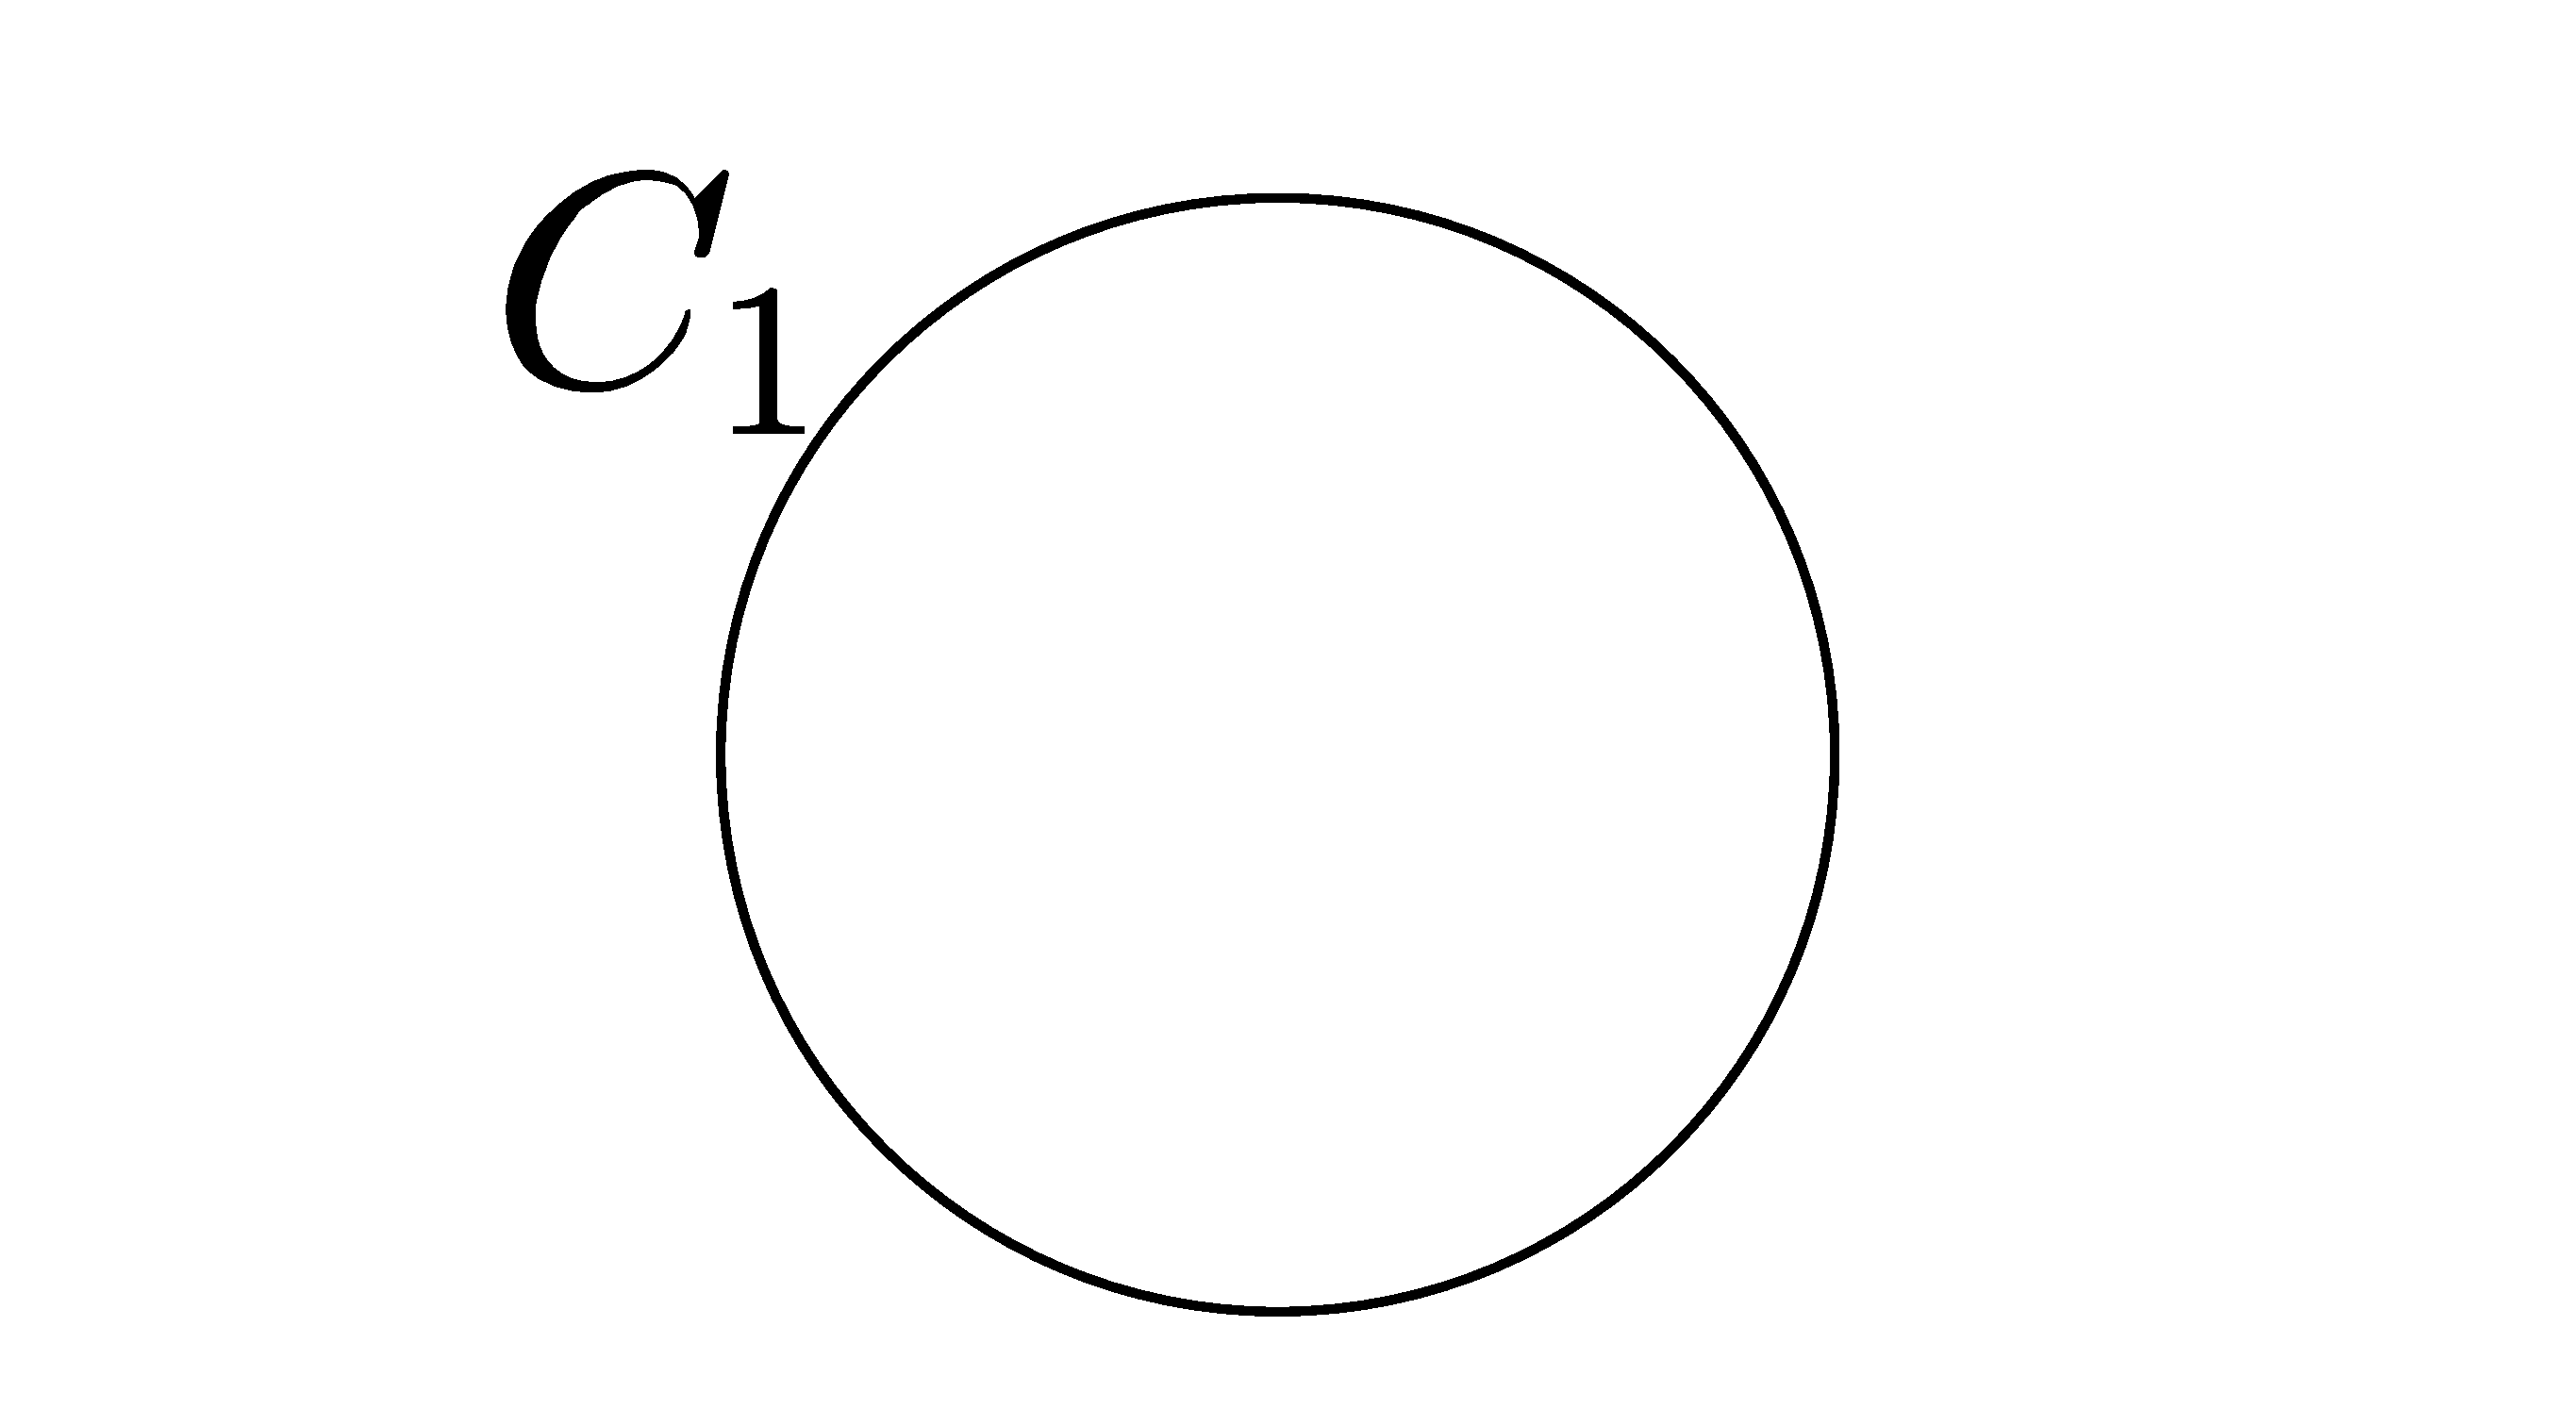
\includegraphics[scale=.065]{Graficos/elipse.eps}}
	\subfigure[Hipérbola]{
\includegraphics[scale=.028]{Graficos/hiperbola.eps}}
	\subfigure[Parábola]{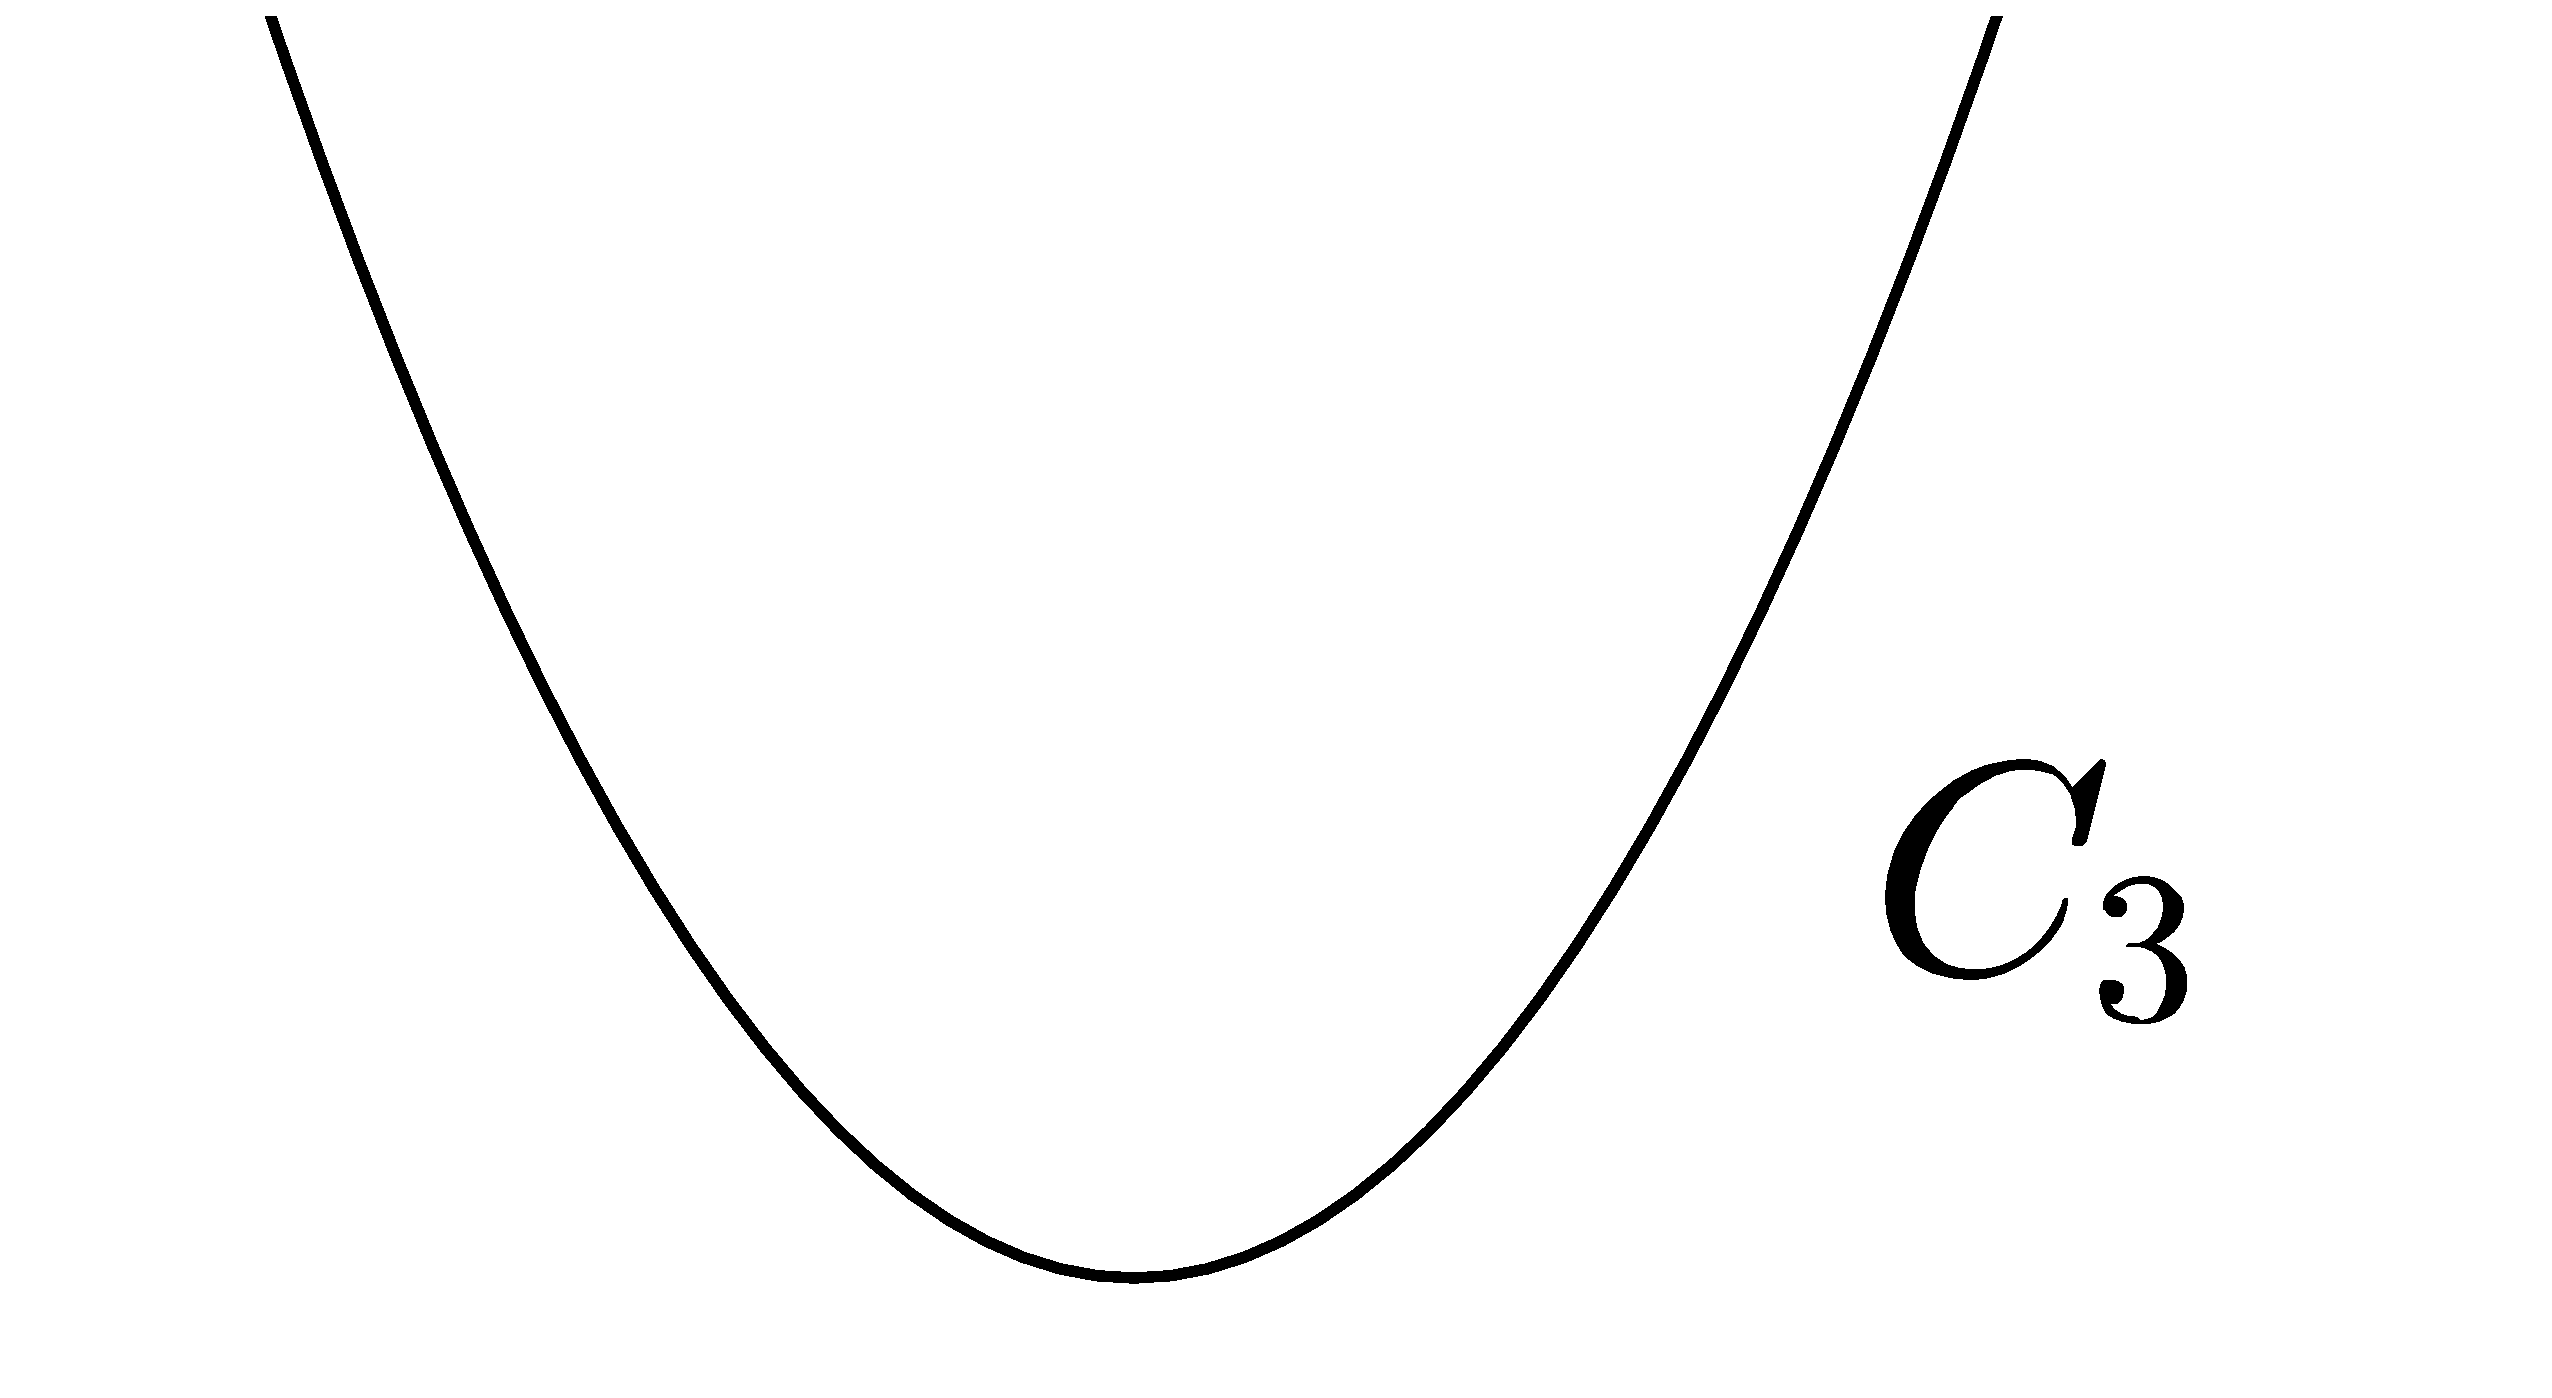
\includegraphics[scale=.06]{Graficos/parabola.eps}}
	\caption{Ilustración de los tipos de cónicas.}
	\label{C7_img_tiposConicas}
\end{figure}
Para que esta clasificación no resulte demasiado abstracta al lector, pongamos un ejemplos de cónicas de cada uno de los tipos.
\begin{exa}[Elipse]
	\label{C8_exa_elipse}
	Consideramos la cónica dada por la siguiente ecuación:
	\[C:x^2+y^2-z^2=0\]
	Intersequemos la cónica con la recta $l_\infty:z=0$ para poder clasificarla.
	\[\left.\begin{array}{c}
	x^2+y^2-z^2=0\\
	z=0
	\end{array}\right\}\leadsto x^2+y^2=0\]
	Es claro que la única solución a esta ecuación es el punto $(0,0,0)$, sin embargo, el rayo engendrado por este vector no está definido. Por ende, no hay ningún rayo (punto proyectivo) de la cónica que sea, a la vez, un rayo de la recta del infinito. Por ende, esta cónica es una elipse.
\end{exa}
\begin{exa}[Hipérbola]
	Clasifiquemos la cónica de ecuación:
	\[C:X^2-Y^2=1\]
	Antes de que cunda el pánico, nótese que esta ecuación nos viene dada en forma ``deshomogeneizada'' (si no no sería la ecuación de una cónica). Al homogeneizarla nos queda algo bastante más familiar:
	\[C:x^2-y^2-z^2=0\]
	Calculemos los puntos de corte con $z=0$:
	\[\left.\begin{array}{c}
	x^2-y^2-z^2=0\\
	z=0
	\end{array}\right\}\leadsto x^2=y^2\]
	Tomando raíces cuadradas y considerando todos los casos necesarios obtemos como soluciones los puntos de la forma:
	\[\begin{array}{cc}
	\class{(\lambda,\lambda,0)}=(1:1:0)\qquad & \qquad \class{(\lambda,-\lambda,0)}=(1:-1:0)
	\end{array}\]
	Por ende, la cónica $C$ tiene dos puntos de corte con la recta del infinito, esto significa que es de tipo hiperbólico.
\end{exa}
\begin{exa}[Parábola]
	Se nos da la siguiente cónica en forma no homogénea:
	\[C:Y=X^2\]
	Calculemos (tras homogeneizar) los puntos de corte de la misma con $l_\infty$.
	\[\left.\begin{array}{c}
	zy-x^2=0\\
	z=0
	\end{array}\right\}\leadsto x^2=0\]
	Teniendo en cuenta esto, los puntos que cumplen las restricciones impuestas por ambas ecuaciones son los de la forma $(0,\lambda,0)$ (los cuales, además, son solución doble). Estos generan un único rayo. Por ende, la cónica y la recta del infinito únicamente se cortan en un punto. Esto es lo mismo que decir que $C$ es una parábola.
\end{exa}
\section{Matriz de una Cónica}
Vamos a reescribir de una forma especialmente cómoda el polinomio asociado a una cónica. No es necesario memorizar como un loro el proceso de transformación que realizaremos a continuación, ya que, en breve, encontraremos una forma más rápida y simple de hacerlo.
\begin{multline}
	F(x,y,z)=ax^2+by^2+cz^2+2fyz+2gxz+2hxy=\\
	=x(ax+hy+gz)+y(by+fz+hx)+z(cz+fy+gx)
\end{multline}
Expresando todo esto e forma matricial obtenemos (compruébese):
\[F(x,y,z)=\begin{pmatrix}
x & y & z
\end{pmatrix}\begin{pmatrix}
ax+hy+gz\\
hx+by+fz\\
gx+fy+cz
\end{pmatrix}=\begin{pmatrix}
x & y & z
\end{pmatrix}\begin{pmatrix}
a & h & g\\
h & b & f\\
g & f & c
\end{pmatrix}\begin{pmatrix}
x\\
y\\
z
\end{pmatrix}\]
De forma abreviada (abusando de notación) usualmente escribiremos:
\[F(X)=X^tAX\]
A la matriz $A$ se la denomina \ti{matriz de la cónica} asociada al polinomio $F$. No mucho más adelante (simplemente por comodidad) desarrollaremos el concepto de \ti{matriz de una cuádrica} en general.

\begin{obs}[Regla Mnemotécnica]
	Una regla mnemotécnica para acordarse de los coeficientes de esta matriz es símplemente notar que es una matriz simétrica en cuya diagonal están los coeficientes asociados a monomios con variables al cuadrado. Para rellenar el ``triángulo'' superior (y por tanto el inferior) basta con recorrer dicho triángulo desde su vétice inferior en sentido antihorario y colocar allí los coeficientes asociados a los monomios de variables $yz$, $xz$ y $xy$ respectivamente. Este truco tiene realmente poca importancia, ya que aprenderemos a calcular esta matriz una forma bastante mecánica.
\end{obs}

\begin{obs}[Matriz de una Cónica y Formas Bilineales]
	\label{C8_obs_bilineal}
	El lector que aún guarde en su mente bastantes remanentes de lo que cursó en su día de álgebra lineal se habrá dado cuenta de la relación entre el polinomio asociado a una cónica y las formas bilineales. De hecho, los polinomios asociados a cónicas \tb{son} formas bilineales simétricas. Además, lo que nosotros llamamos matriz de la cónica, es en realidad la matriz asociada a la forma bilineal.
	
	Sin embargo, una forma bilineal podía tener varias matrices asociadas (aunque solo una de ellas simétrica). Reflexionemos un poco sobre esto.
	
	Consideremos que la matriz $A$ es la asociada al polinomio $F$ (asociado a cierta cónica). Entonces, la imagen de un vector por el polinomio se escribe de la forma:
	\[F(X)=X^tAX\]
	Es ahora cuando traemos a colación un viejo y olvidado resultado de álgebra lineal que afirma que cualquier matriz puede ser descompuesta en una parte simétrica y otra antisimétrica de la siguiente manera:
	\[\begin{array}{ccc}
	A=A_s+A_a\qquad &\qquad A_s=\frac{1}{2}(A+A^t)\qquad &\qquad A_a=\frac{1}{2}(A-A^t)
	\end{array}\]
	En definitiva:
	\[F(X)=X^tAX=X^t(A_s+A_a)X=X^tA_sX+X^tA_aX\]
	Notemos que $X^tA_aX$ es un simple numeraco, luego coincide con su traspuesto:
	\[X^tA_aX=(X^tA_aX)^t=-X^tA_aX\sii X^tA_aX=0\]
	En conclusión, la parte antisimétrica de la matriz de una forma bilineal sólo introduce ruido y confusión. Ese es el motivo por el cual construimos (con una astucia en principio ajena al lector) una matriz simétrica como matriz de la cónica.
\end{obs}
Tras la observación \ref{C8_obs_bilineal} ya estamos en disposición de definir el concepto de \ti{matriz asociada a una cuádrica} como la matriz asociada a la forma bilineal simétrica que constituye su polinomio $F$ asociado.

Tras toda esta literatura, enunciemos y demostremos el prometido resultado que nos ayudaría a calcular de forma sencilla la matriz asociada a una cuádrica en general.
\begin{lem}[Matriz Asociada y Matriz Hessiana]
	\label{C8_lem_Hessiana}
	Dada una cuádrica $C$, su matriz asociada $A$ (simétrica) es única.

Además se tiene que: \[A=\frac{1}{2}\mathrm{Hess}(F)\]
Donde $F$ es el polinomio asociado a la cuádrica y $\mathrm{Hess}(F)$ su matriz Hessiana correspondiente.
\end{lem}
\begin{proof}
Demostremos en primer lugar el ``además'', obteniendo trivialmente el resto.

Consideremos el polinomio $F$ asociado a la cuádrica. Como vimos anteriormente, este polinomio admite la forma matricial:
\[F(X)=X^tAX\]
Nuestro objetivo es hallar una expresión única para los coeficientes $a_{ij}$ de la matriz $A$ de la cuádrica. Ayudados por el enunciado de nuestro problema (sabemos que nos tiene que salir la matriz Hessiana del polinomio $F$).

Para el lector que se haya saltado alguna clase de cálculo diferencial en varias variables, recordamos que la matriz Hessiana de una función $F:\C^n\to\C$ (en un punto genérico en el que admita derivadas parciales segundas) es:
\[\mathrm{Hess}(F)=\begin{pmatrix}
\frac{\partial F}{\partial x_1x_1} & \cdots &\frac{\partial F}{\partial x_nx_1}\\
\vdots & \ddots & \vdots\\
\frac{\partial F}{\partial x_1x_n} & \cdots & \frac{\partial F}{\partial x_nx_n}
\end{pmatrix}\]

Asimismo, cabe mencionar que si dicha función $F$ admite derivadas parciales segundas continuas en un punto, entonces la matriz Hessiana es simétrica. Esto es debido al llamado Teorema Mágico de Schwarz.

Para nuestra fortuna, los polinomios en general, y los polinomios asociados a cuádricas en particular, son funciones de clase infinito sobre todo su conjunto de definición, esto es, admiten derivadas parciales continuas de orden arbitrario en cualquier punto, luego su matriz Hessiana es siempre simétrica.

Hallemos pues un coeficiente arbitrario de la matriz Hessiana derivando dos veces $F$ respecto de las variables $x_i$ y $x_j$. Apoyándonos en la expresión matricial que tenemos, podemos ver el polinomio como el producto de dos matrices (matriz fila por matriz columna) que es fácilmente expresable como la siguiente suma (los corchetes son simplemente notacionales).
\[F(X)=(X^t)(AX)=\sum_{k=1}^{n}\left[x_k\left(\sum_{l=1}^{n}a_{kl}x_l\right)\right]\]
Derivando concuidado obtenemos:
\begin{multline}
	\frac{\partial F(x_1,\dots,x_n)}{\partial x_j\partial x_i}=\frac{\partial}{\partial x_j}\left(\frac{\partial F(x_1,\dots,x_n)}{\partial x_i}\right)=\\=\frac{\partial}{\partial x_j}\left(\sum_{k\not= i}^{n}\left[x_k\frac{\partial}{\partial x_i}\left(\sum_{l=1}^{n}a_{kl}x_l\right)\right]+\left(\sum_{l=1}^{n}a_{il}x_l+x_ia_{ii}\right)\right)=\\
	=\frac{\partial}{\partial x_j}\left(\sum_{k\not=i}^{n}x_ka_{ki}+x_ia_{ii}+\sum_{l=1}^{n}a_{il}x_l\right)=\\=\frac{\partial}{\partial x_j}\left(\sum_{k=1}^{n}x_ka_{ki}+\sum_{l=1}^{n}a_{il}x_l\right)=a_{ji}+a_{ij}=2a_{ij}
\end{multline}
Por ende, cada coeficiente de la matriz Hessiana es el doble del coeficiente correspondiente de la matriz de la cuádrica.

Como las derivadas parciales son, al fin y al cabo, límites, estas son únicas, luego la matriz de una cuádrica es única. Además, de esta forma, tenemos un procedimiento efectivo y mecánico para calcularla.
\end{proof}
Pongamos algún ejemplo para que el lector ponga en valor la utilidad de la caracterización ofrecida por el lema \ref{C8_lem_Hessiana}.
\begin{exa}[Cálculo de la Matriz de una Cuádrica]
	Dadas las siguientes cónicas, calculemos automáticamente sus matrices asociadas obteniendo la mitad de las matrices Hessianas de los polinomios.
	\[\begin{array}{c}
	C_1:x^2+y^2+z^2=0\leadsto\frac{1}{2}\begin{pmatrix}
	1 & 0 & 0\\
	0 & 1 & 0\\
	0 & 0 & 1
	\end{pmatrix}\\
	C_2:x^2+y^2+2z^2=0\leadsto\frac{1}{2}\begin{pmatrix}
	1 & 0 & 0\\
	0 & 1 & 0\\
	0 & 0 & 2
	\end{pmatrix}
	\end{array}\]
\end{exa}
A continuación veremos que dos polinomios ``proporcionales'' generan la misma cuádrica.

Esto es importante por muchos motivos. El primero, y el más evidente a simple vista, es que para calcular la matriz de una cuádrica ya no hace falta multiplicar la matriz Hessiana del polinomio $F$ por ningún factor. Bastaría considerar que la cuádrica está generada por el polinomio $2F$. Veamos esto con detalle.
\begin{obs}[Polinomios Proporcionales]
	\label{C8_obs_proporcionales}
	Dado un polinomio $F$ (con las restricciones habituales), resulta evidente que el conjunto de ceros de $F$ es igual al conjunto de ceros del polinomio $\lambda F$ para cierto $\lambda\in\C$ no nulo.
\end{obs}
Otro de los motivos por los que la observación \ref{C8_obs_proporcionales} es de gran importancia, es que, como veremos (dejándonos pendiente algún detalle), el conjunto de las cúadricas proyectivas de $\proy(\C^n)$ puede verse como un espacio proyectivo $\proy(\C^k)$ para cierto $k$ (que calcularemos explícitamente). 
\begin{obs}[Pseudolema de la Correspondencia]
	\label{C8_obs_pseudoCorrespondencia}
	Es evidente que la relación de proporcionalidad de polinomios es una relación de equivalencia a la que denotaremos $\sim$. Consideremos pues el conjunto cociente de los polinomios (compuestos únicamente por monomios de grado $2$, a los que denotaremos por $\mc{P}$) ``módulo'' la relación de equivalencia $\sim$. A este conjunto lo denotaremos:
	\[\mc{F}:=\frac{\mc{P}}{\sim}\]
	Es una fácil comprobación (que se deja al lector) demostrar que el conjunto de los polinomios con nuestras restricciones habituales es un espacio vectorial (cuya dimensión desconocemos por el momento). Por ello, el conjunto $\mc{F}$ no es más que el espacio proyectivo asociado a $\mc{P}$. Por este motivo, denotaremos por $\class{F}$ a los elementos de $\mc{F}$.
	
	Es evidente (por definición) que la siguiente aplicación es sobreyectiva:
	\[\begin{array}{c}
	\mc{F}\stackrel{\Psi}{\to}\mc{C}\\
	\class{F}\mapsto\phi(F)
	\end{array}\]
	Donde $\mc{C}$ representa el conjunto de las cuádricas del espacio proyectivo complejo $n+1$ dimensional y $\phi$ es la aplicación que a cada polinomio le asocia su conjunto de ceros.
	
	Resulta ser también cierto (como veremos más adelante) que la aplicación $\Psi$ es inyectiva, pudiendo identificar canónicamente al conjunto de cuádricas $\mc{C}$ con el espacio proyectivo $\mc{F}$.
\end{obs}
	Hagamos un pequeño (gran) acto de fe y consideremos probado que la aplicación $\Psi$ definida en la observación \ref{C8_obs_pseudoCorrespondencia} es (como ya se adelantó) biyectiva. Dando esto por hecho, tratemos de calcular la dimensión de $\mc{P}$.
	\begin{obs}[Dimensión de $\mc{P}$]
		\label{C8_obs_dimension}
		Como ya sabemos, los vectores de $\mc{P}$ son formas bilineales simétricas, y como tales, quedan totalmente determinadas por una matriz simétrica $n\times n$. Es un ejercicio de álgebra lineal comprobar que la aplicación que asociada a cada polinomio $F$ su matriz correspondiente es un isomorfismo de espacios vectoriales.
		
		Esto quiere decir que $\mc{P}$ y el espacio vectorial de las matrices simétricas $n\times n$ tienen la misma dimensión, que es, precisamente, (compruébese) $\frac{n^2+n}{2}:=\xi$.
		
		Por ende, $\mc{P}$ es isomorfo a $\C^\xi$. Como las cuádricas de $\C^n$ se confunden con $\proy(\mc{P})\cong\proy(\C^\xi)$, habitualmente se dirá que las cuádricas de $\C^n$ \ti{son} un $\proy(\C^\xi)$.
	\end{obs}
	Un resultado cuanto menos sorprendente, y bonito, que se desprende de forma inmediata de la observación \ref{C8_obs_dimension}, es que las cónicas del plano proyectivo complejo son un espacio proyectivo de dimensión $5$. En efecto:
	\[\xi=\frac{3^2+3}{2}-1=5\]
	No debemos olvidarnos de que queda pendiente la demostración de que cada cuádrica está asociada a un único rayo de polinomios.
\section{Determinaciones de una Cónica}
El objetivo de esta sección será demostrar que, bajo ciertas condiciones, cinco puntos del espacio proyectivo $\proy^2$ determinan unívocamente una cónica.
\subsection{Cónicas como Producto de dos Rectas}
Dadas dos rectas de $\proy^2$, a las que $l$
\section{Deshomogeneizaciones de una Cónica}